% fig_confidence.tex
% Confidence score c vs 3rd harmonic injection I_h3
% Data from TR-21 (no_fault scenario): fixed DFT drops to 0.37, pre-filter stays at 1.0
% Also shows int_fault scenario (fixed stays adequate, pre-filter improves)
% gamma_min = 0.80 threshold line
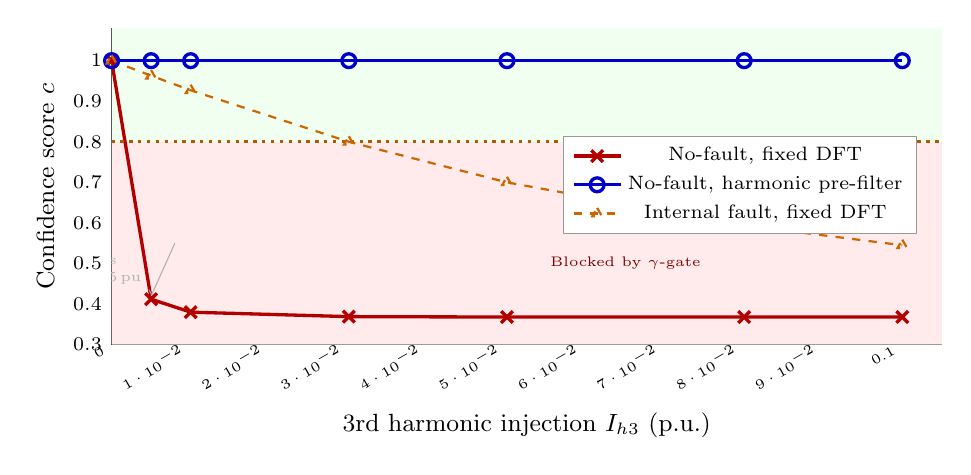
\begin{tikzpicture}
\begin{axis}[
  width=\columnwidth, height=5.6cm,
  xlabel={3rd harmonic injection $I_{h3}$ (p.u.)},
  ylabel={Confidence score $c$},
  xmin=0, xmax=0.105,
  ymin=0.30, ymax=1.08,
  xtick={0,0.01,0.02,0.03,0.04,0.05,0.06,0.07,0.08,0.09,0.10},
  xticklabel style={font=\tiny,rotate=30,anchor=east},
  ytick={0.3,0.4,0.5,0.6,0.7,0.8,0.9,1.0},
  grid=both,
  grid style={gray!22,line width=0.3pt},
  tick label style={font=\scriptsize},
  label style={font=\small},
  legend style={at={(0.97,0.35)},anchor=south east,
                font=\scriptsize,fill=white,draw=black!40},
  clip=true]

  % Reject region (c < gamma_min)
  \addplot[fill=red!8,draw=none,forget plot]
    coordinates {(0,0.30)(0.105,0.30)(0.105,0.80)(0,0.80)} \closedcycle;
  \node[font=\tiny,red!50!black] at (axis cs:0.065,0.50) {Blocked by $\gamma$-gate};

  % Accept region
  \addplot[fill=green!6,draw=none,forget plot]
    coordinates {(0,0.80)(0.105,0.80)(0.105,1.08)(0,1.08)} \closedcycle;

  % No-fault: fixed DFT (drops below gate at I_h3>=0.005)
  \addplot[red!70!black,very thick,mark=x,mark size=3pt]
    coordinates {
      (0.000, 1.000)
      (0.005, 0.412)
      (0.010, 0.380)
      (0.030, 0.369)
      (0.050, 0.368)
      (0.080, 0.368)
      (0.100, 0.368)
    };
  \addlegendentry{No-fault, fixed DFT}

  % No-fault: adaptive pre-filter (stays at 1.0)
  \addplot[blue!80!black,very thick,mark=o,mark size=2.5pt]
    coordinates {
      (0.000, 1.000)
      (0.005, 1.000)
      (0.010, 1.000)
      (0.030, 1.000)
      (0.050, 1.000)
      (0.080, 1.000)
      (0.100, 1.000)
    };
  \addlegendentry{No-fault, harmonic pre-filter}

  % Int-fault: fixed DFT (degrades but stays above gate until I_h3~0.03)
  \addplot[orange!80!black,thick,dashed,mark=triangle,mark size=2pt]
    coordinates {
      (0.000, 1.000)
      (0.005, 0.963)
      (0.010, 0.927)
      (0.030, 0.800)
      (0.050, 0.700)
      (0.080, 0.594)
      (0.100, 0.545)
    };
  \addlegendentry{Internal fault, fixed DFT}

  % gamma_min threshold
  \draw[orange!70!black,very thick,dotted]
    (axis cs:0,0.80) -- (axis cs:0.105,0.80)
    node[right,font=\tiny,orange!80!black]{$\gamma_{\min}=0.80$};

  % Annotation: gate closes at 0.005 pu
  \draw[->,gray!60,thin]
    (axis cs:0.008,0.55) -- (axis cs:0.005,0.42)
    node[above left,font=\tiny,gray!60,align=left]{gate closes\\$I_{h3}{=}0.005$\,pu};

\end{axis}
\end{tikzpicture}
